\chapter{Design}
\label{design}

\textbf{General design:} semi-centralized, hierarchical peer-to-peer system utilizing the pipe-flow architecture pattern
in which leaf (sensor) nodes of the hierarchy collect data, filter out extraneous data, and send it up the pipe to an
aggregate node which subsequently filters out more data and sends it up to another aggregate or root node.

\dcamp was designed to be simple and only add complexity where needed. This allows, for example, for quick and easy,
large scale testing. Additionally, in order to be transparent, minimizing network traffic was important.

\section{Requirements}

\subsection{Functional}

\begin{enumerate}

\item Configuration
      \begin{itemize}
      \item instantiation, administration
      \item topology coordination
      \item metric collection spec.
      \end{itemize}

\item Metric Collection
      \begin{itemize}
      \item \dcamp API on top of CAMP
      \item filters (at various levels), thresholds
      \item aggregation of metrics across nodes
      \item output to log file
      \end{itemize}

\item Fault Tolerance
      \begin{itemize}
      \item simple rules to handle failures
      \end{itemize}

\end{enumerate}

\subsection{Fault Tolerance}

\begin{enumerate}

\item Topology MUST sustain brief network disconnectivity of any node.
\item Sensor nodes MUST be allowed to enter/exit topology at any time.
\item Root/Collector nodes (i.e. parents) MUST failover in case of extended disconnectivity.
      \begin{itemize}
      \item Loss of previously collected data SHOULD be minimized during failover.
      \end{itemize}
\item Management node SHOULD be allowed to enter/exit topology at any time.

\end{enumerate}

\subsection{Testing}

\begin{itemize}

\item \textbf{Transparency:} \dcamp SHOULD introduce negligible performance impact on sensor nodes.
\item \textbf{Accuracy:} \dcamp MUST accurately report metrics/performance of sensor nodes (individual and aggregated).
\item \textbf{Scalability:} \dcamp SHOULD maintain its transparency and accuracy as it scales (i.e. the number of sensor
      nodes increases).
\item \textbf{Fault Tolerance:} \dcamp MUST successfully handle entrance/exit of any node(s) in the system.

\end{itemize}

\section{\dcamp Roles and Services}
\label{roles_and_services}

The \dcamp distributed system is comprised of one or more nodes each running one or more roles. Each role--a published,
remotely accessible interface--provides one or more sets of functionality. Each set of functionality is known as a
service.

\subsection{Services}

\begin{itemize}

\item \textbf{Node}---rudimentary \dcamp functionality; handles topology communication, heartbeat monitoring, and failure
      recovery.
\item \textbf{Sensor}---local performance metric gathering; essentially the \dcamp layer on top of the OS and hardware
      performance APIs (accessed via CAMP).
\item \textbf{Filter}---performance metric filtering; provides throttling and thresholding of metrics.
\item \textbf{Aggregation}--—performance metric aggregation; provides collection of and calculation on metrics from
      multiple sensors and/or collectors.
\item \textbf{Management}--—primary entry-point for end-user control of \dcamp distributed system; this is the \dcamp
      instrument panel, providing basic administration functions (e.g. start, stop, etc.).
\item \textbf{Configuration}--—complete or partial configuration replication; provides topology and configuration
      distribution.

\end{itemize}

\subsection{Roles}

The \textit{Base} role must be running on each node for it to be part of the \dcamp distributed system. In this document,
a ``Base node'' is defined as a \dcamp node which has not yet been configured, i.e. it has not joined a running \dcamp
system.

The \textit{Metric} role runs on the nodes from which performance metrics should be collected. The \textit{Collector}
role acts as an aggregation point in the system, combining performance data from multiple \textit{Metric} (and
\textit{Collector}) nodes and providing additional aggregated performance metrics.

There is only one \textit{Root} role active in the system; it acts as the master copy of the \dcamp configuration and
sole user-interface point. The \textit{Root} role is not strictly attached to any given node in the system. Rather, the
\textit{Root} role may dynamically move to any first-level \textit{Collector} node if the current \textit{Root} node
fails.

Depending on the use case and desired system performance, an administrator may choose to split roles across multiple
nodes or collapse them onto a single node. For example, a single node may act as \textit{Metric}, \textit{Collector},
and \textit{Root} for smaller systems while larger systems would employ dedicated \textit{Collector} nodes.

\subsection{Role-to-Service Mappings}

Table \ref{tab:role_to_services} lists the roles which can be ``published'' by a \dcamp node and the services which they
implement.

\begin{table}
\begin{tabular}{l l}

\hline
\textbf{Role} & \textbf{Service(s)} \\
\hline

Root & Management, Aggregation, Filter, Configuration (Full) \\

Collector & Aggregation, Filter, Configuration (Full) \\

Metric & Sensor, Filter, Configuration (Partial) \\

Base & Node \\

\end{tabular}
\caption{Role to Service Mappings}
\label{tab:role_to_services}
\end{table}

\section{Fault Tolerance}

\subsection{Heartbeating (Detecting Disconnections)}

Disconnections are detected via a lack of messages, e.g. missed X consecutive messages or no messages received after D
seconds.

\begin{itemize}
\item Metric nodes MUST detect when their parent (Collector) node disconnects. (\hyperref[algor_promo]{Promotion Algorithm})
\item The Root node MAY detect when a Collector node disconnects. (\hyperref[algor_promo]{Promotion Algorithm})
\item Collector nodes MUST detect when the Root node disconnects. (\hyperref[algor_elect]{Election Algorithm})
\item The Root node MUST detect when a Metric node rejoins the system. (\hyperref[algor_remind]{Reminder Algorithm})
\end{itemize}

LATER

\begin{itemize}
\item should the configuration TTL be used somehow?
      \begin{itemize}
      \item alternatively, this could be based on configuration entry TTL expiration.
      \item collector-to-collector heartbeating? not needed, since these TTLs will come from the root (via the data protocol)
      \item ttl used to know which first-level collectors are root-eligible?
      \end{itemize}
\item heartbeats are sent from first-level collectors to root or all collectors?
\item does a collector need to know when a metric node disconnects? no.
\end{itemize}

\subsection{Reminder Algorithm (Metric Node Recovery)}
\label{algor_remind}

Metric nodes can leave and enter the \dcamp system at any time. When they rejoin, they should be placed back into the
same location within the topology so as to maintain as much consistency within the performance data as possible.

The crux of this algorithm is the group definitions within the \dcamp configuration: nodes are always defined to be
within a group, and the groups define the network topology. Essentially, this algorithm is incorporated into the
Topology protocol; no additional work is necessary.

\begin{enumerate}
\item Sensor node rejoins the system with \texttt{POLO} response to Root node's \texttt{MARCO} message.
\item Root node detects Metric node is already part of \dcamp system.
\item Root node (re)sends \texttt{ASSIGN} message to Metric node.
\end{enumerate}

\subsubsection{DETECTION}

Detecting when a Metric node disconnects is not necessary. Rather the Root node only needs to detect when a Metric node
rejoins the \dcamp system, comparing the Metric node's UUID to the UUID already saved in the topology.

\subsubsection{QUESTIONS}

\begin{itemize}
\item How does this account for new nodes which have been assigned to Collector node since this Metric node
      disconnected? Can the Collector node become overloaded, or is this already accounted for with the configuration
      groups?
\end{itemize}

\subsection{Promotion Algorithm (Collector Node Recovery)}
\label{algor_promo}

As with the Reminder Algorithm, this recovery relies heavily on the \hyperref[proto_topo]{Topology Management Protocol}.
When a Metric node, M, detects its Collector node, C, is down, 

\begin{enumerate}
\item M sends an \texttt{SOS} message to the Root node, R.
\item If R has received an \texttt{SOS} message from more than 1/3 of C's group, the algorithm proceeds as per below.
\end{enumerate}

When the Root node, R, detects one of the Collector nodes has disconnected,

\begin{enumerate}
\item R broadcasts a \texttt{STOP} message to all nodes within C's group and clears the groups configuration from the
      \dcamp system.
\item R then broadcasts a \texttt{MARCO} message and begins rebuilding the group topology via the Topology protocol.
\end{enumerate}

\subsubsection{DETECTION}

M will use the \hyperref[proto_config]{Configuration Replication Protocol} (\texttt{HUGZ}) to detect when C disconnects.
R will use the \hyperref[proto_data]{Data Flow Protocol} (\texttt{METRIC(type='HUGZ')}) to detect when any of its
Collector nodes has disconnected. That is, if M or R receives no messages from C within D seconds, C is considered
disconnected.

\subsection{Election Algorithm (Root Node Recovery)}
\label{algor_elect}

This recovery algorithm is based on the bully algorithm\cite{needed}. Only Collector nodes participate in the election,
initiated when a Collector node, C, detects the Root node, R, is down.

\begin{enumerate}
\item C sends \texttt{WUTUP} message to all nodes whose UUID is higher than its own, expecting a \texttt{YO} message in
      response.
\item If C does not receive any \texttt{YO} messages,
      \begin{enumerate}
      \item C declares victory by sending \texttt{IWIN} message to all nodes, and
      \item C waits W seconds before transitioning to become the Root, allowing for another node to replace it as Root
            via a separate election.
      \end{enumerate}
\item If C receives a \texttt{YO} message,
      \begin{enumerate}
      \item C waits for W seconds to receive an \texttt{IWIN} message from another node whose UUID is higher than its
            own.
      \item If no \texttt{IWIN} message is received, C resends its \texttt{WUTUP} message and goes through the election
            process again.
      \end{enumerate}
\end{enumerate}

Additionally,

\begin{itemize}
\item If C receives a \texttt{WUTUP} message from a node whose UUID is lower than its own, C responds with a \texttt{YO}
      message and then starts its own election.
\item If C receives an \texttt{IWIN} message from a node whose UUID is lower than its own, C immediately begins a new
      election.
\end{itemize}

\subsubsection{DETECTION}

C will use the \hyperref[proto_config]{Configuration Replication Protocol} (\texttt{HUGZ}) to detect when R disconnects.
That is, if C receives no message from R within D seconds, R is considered disconnected.

\subsubsection{QUESTIONS}

\begin{itemize}
\item Is there a difference between starting a new election and resending the initial \texttt{WUTUP} message? Is there
      an optimization to be found by uniquely ID'ing each election?
\item Can this algorithm be optimized w.r.t. the number of messages sent?
\end{itemize}

\section{\dcamp Operation}

\subsection{Sequence of \dcamp Operation}
\label{operation_sequnce}

The following steps describe how the \dcamp system is turned on. The Base nodes (other than the node assigned to be the
Root) can be started at any time by using the \dcamp CLI, before or after the Root node is initialized. It is expected
these Base nodes are managed by a watchdog utility which automatically restarts the node if it exits for any reason.

\begin{figure}[H]
\vspace{+10pt}
\begin{lstlisting}[language=bash,frame=single,basicstyle=\footnotesize\ttfamily]
#!/usr/bin/env bash
while [ true ]
do
    dcamp base --address localhost:56789
done
\end{lstlisting}
\vspace{-10pt}
\caption{Sample Watchdog Script}
\label{fig:sample_watchdog}
\end{figure}

\begin{enumerate}

\item User promotes a Root node via the \dcamp CLI, specifying a configuration file and a Base node's address.
\item Root node connects to each Base node and begins the ``discover'' \hyperref[proto_topo]{Topology Protocol}.
\item Base nodes join the \dcamp system at any time, being assigned as Collector or Metric nodes in the topology.

\item \dcamp runs in a steady state, nodes entering or exiting the system at any time.

      \begin{itemize}
      \item Performance counters are sampled, filtered, reported, and logged by the Metric nodes at regular intervals
            according to the \hyperref[imp_configuration]{\dcamp Configuration}.
      \item Performance counters received from child nodes are aggregated, filtered, reported, and logged by Collector
            nodes at regular intervals according to the \dcamp Configuration.
      \item Performance counters received from child nodes are aggregated and logged by Root node for later processing
            (e.g. graphing metrics during a test scenario or correlating statistics with a distributed event log).
      \end{itemize}

\item User stops \dcamp by using the \dcamp CLI command.
\item Root node begins the ``stop'' Topology Protocol.
\item Collector and Metric nodes exit the topology and revert to Base nodes.
\item Root node exits, reverting to Base node.

\end{enumerate}

\subsection{Threading Model}

As mentioned above as the first and third steps of \dcamp operation, a Base node can transform into one of the three
active \dcamp roles: Root, Collector, or Metric. This transformation is actually the Base role (via the Node service)
launching and managing another Role internally. This interaction is depicted in Figure
\ref{fig:node_role_service_image}.

\begin{figure}[H]
    \centering
    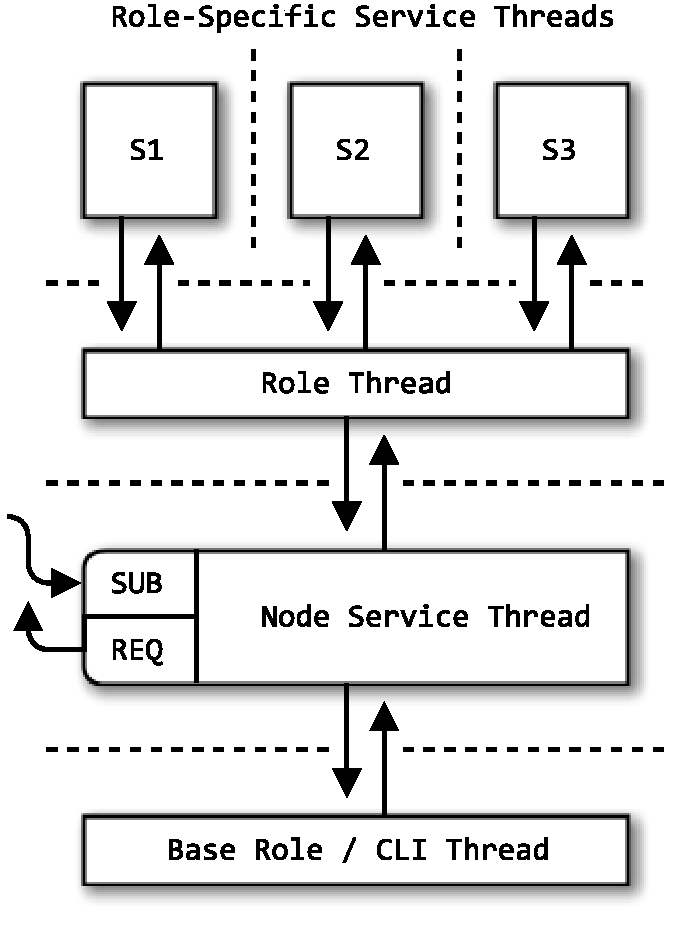
\includegraphics[scale=0.5]{node-role-service.pdf}
    \caption[Node, Role, Services Threading Model Diagram]
            {Node, Role, Services Threading Model Diagram: Thread boundaries are represented by dashed lines. Except for
	     the Node service's \texttt{SUB} and \texttt{REQ} sockets, all arrows represent \texttt{PAIR} socket
	     communication.}
    \label{fig:node_role_service_image}
\end{figure}

When a Base node is running, only the bottom two threads (the Base role and the Node service) are active. Once it
receives an assignment from the ``discover'' Topology Protocol or the \dcamp CLI, the Node service launches an
appropriate Role thread which, in turn, launches one or more Role-specific service threads.

All communication between the roles and services occurs across \texttt{PAIR} control sockets. There are also various
service-to-service communications which occur via \texttt{inproc} transport sockets (e.g. the internal
\hyperref[proto_data]{Data Flow Protocol}) and shared memory data structures (e.g. the Configuration service).

Also mentioned in section \ref{operation_sequnce} as the last two steps, each Role exits and, by doing so, reverts
itself back to a Base node. This is handled just like before, with the Node service receiving a \texttt{STOP} message
via the ``stop'' Topology Protocol and then notifying the internally running Role to shut down. The Role thread then
notifies its service threads, waits for them to finish, then exits.

